\documentclass[10pt,english]{article}
\usepackage[T1]{fontenc}
\usepackage[latin9]{inputenc}
\usepackage[a4paper]{geometry}
\geometry{verbose}
\pagestyle{plain}
\usepackage{babel}
\usepackage{graphicx}

\usepackage{amsmath}
\usepackage{setspace}
\onehalfspacing
\usepackage[unicode=true, pdfusetitle,
 bookmarks=true,bookmarksnumbered=false,bookmarksopen=false,
 breaklinks=false,pdfborder={0 0 1},backref=false,colorlinks=false]
 {hyperref}

\usepackage{fouriernc}
\usepackage{siunitx}
\usepackage{microtype}
\usepackage{nicefrac}

\begin{document}

%\author{Gen Zhang}
\title{Notes on spinal chord structure and development}

\maketitle

Spinal cord forms a pseudo-stratified tissue in which cells are organised in domains which lie parallel along the anterior-posterior (AP) axis. The width of the domains along the dorsal-ventral (DV) axis changes through development, as does the thickness along the apical-basal (AB) axis. The cells move to the apical surface during mitosis, and then move back. Fully differentiated neurons migrate out of the pseudo-stratified layer. Note that there is no clear physiologically defined boundary between the progenitor domains and the mature neurons, e.g. such as the stratified layers in epidermis/oesophagus or a separating membrane. Although there is a slight morphological difference in that progenitors are elongated and post-mitotic cells are more round, having detached from the apical end, the main differentiator is the progenitor marker Sox2; there is also the mature neuron marker p27, but its build up is delayed with respect to the down regulation of Sox2, and so can under-report; as such, we use Sox2 as ground truth.

\begin{figure}[h]
	\begin{center}
		\includegraphics[width=4in]{spinal-chord-anatomy.png}
	\end{center}
	%\label{fig:anatomy}
\end{figure}

In 24 hour EdU incorporation studies, it is observed that the entire progenitor domain is EdU+, as well as some mature neurons. From the number of neurons produced which are EdU- we can infer the number of post-mitotic cells in the progenitor domains at the start of the 24 hour period. A rough count of a Pax7 domain showed that around 30 mature neurons are produced during this period, of which 10 are EdU-; there are around 200 progenitors in the domain to begin with, thus only around $5\%$ of the cells are post-mitotic. However, it is observed that $100\%$ of cells in the progenitor domains express Sox2, implying that it has a moderate decay period. Further, it is observed (based only on two observations) that post-mitosis migration takes around 7 hours, with very little variance; it is also thought that division rates are around 20--30 hours. This is sufficiently long that for accurate statistics, the time spent migrating should not be ignored.

As such, the following model is proposed:

\begin{figure}[h]
	\begin{center}
		\includegraphics[width=4.4in]{division-process-A.png}
	\end{center}
	%\label{fig:division-process-A}
\end{figure}

For a first stab at modelling, it is probably sufficient to treat $\lambda(t)$ as exponential, i.e.\ perfectly stochastic, and $\gamma(t)$ as a $\delta$-distribution, i.e.\ perfectly synchronous.

Notice that if it is the case that the daughters of a progenitor independently make a decision about differentiation, then we expect the relation: $\sqrt{r_2 (t)} = 1 - \sqrt{r_1(t)}$.

At the moment, we have access to various data relating to sections in the transverse (AB/DV) plane, which are around $s = \SI{6}{\micro\metre}$ in thickness. From these sections, it is possible to measure the \textbf{cell density per unit area} $1/a_d$ in the progenitor domains, and the \textbf{number of progenitors and neurons}, $p_d$ and $n_d$, respectively. The domains are also roughly rectangular, and to a certain extent we can assign some \textbf{absolute dimensions} $[DV]_d$ and $[AB]_d$; however, the actual area of the progenitor domains are more accurately measured by $p a$, as opposed to $[DV][AB]$. The absolute dimensions will have more direct impact on signalling.

\begin{figure}[h]
	\begin{center}
		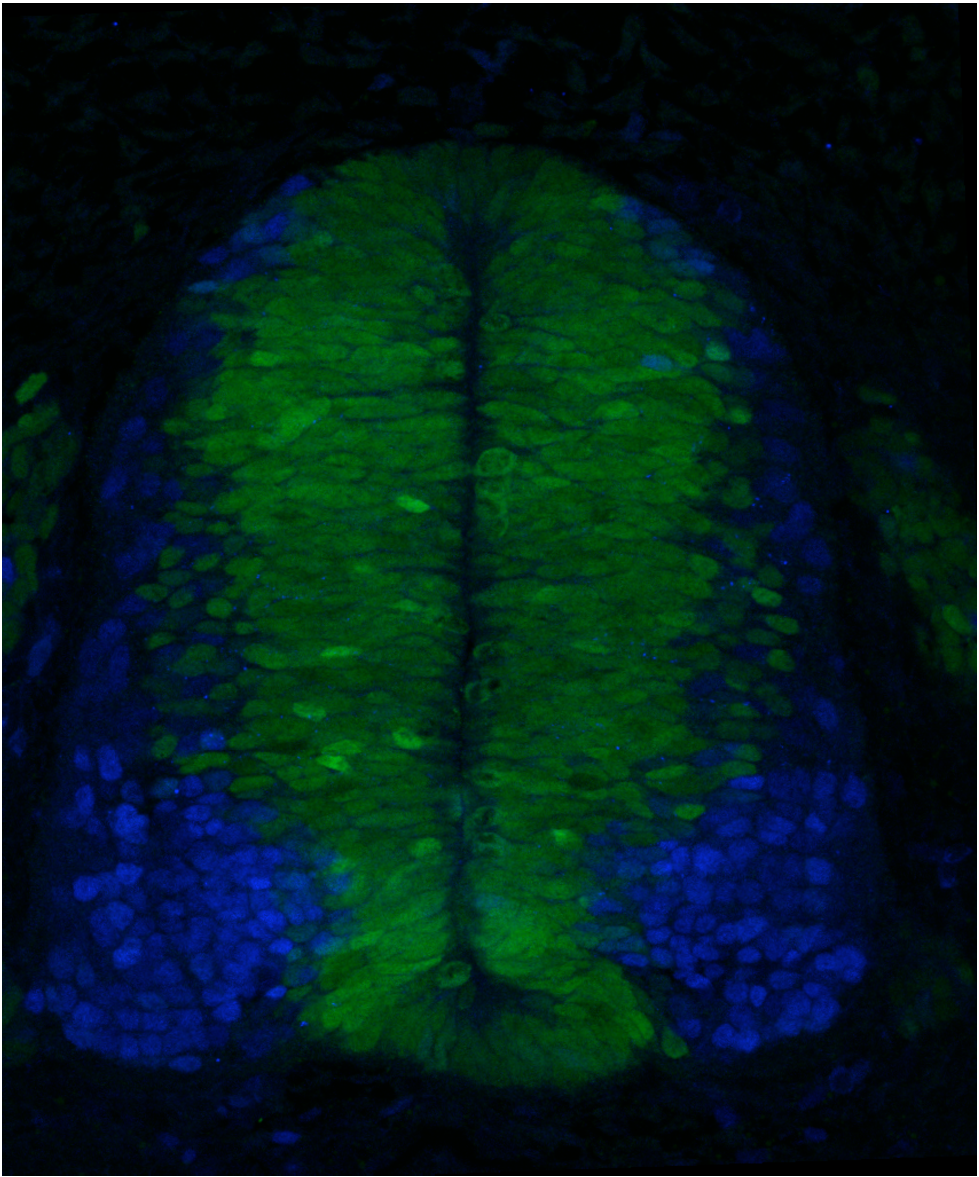
\includegraphics[height=3in]{transverse-stained-sox2-p27.pdf}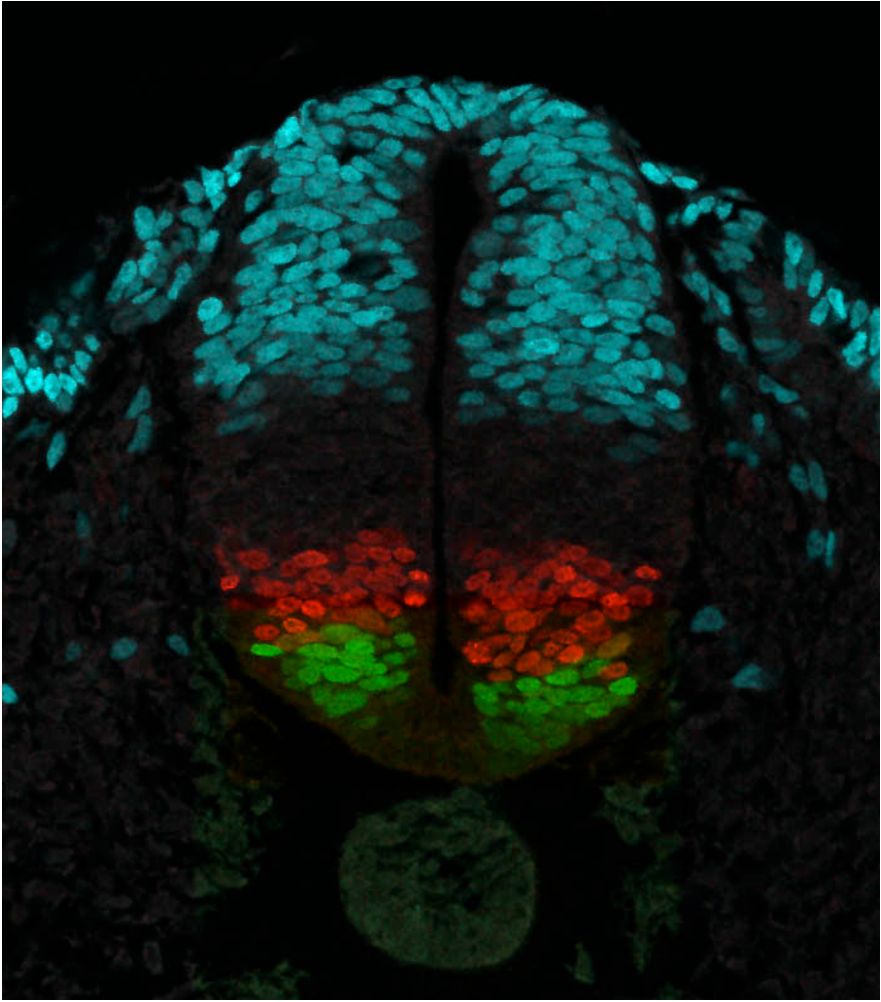
\includegraphics[height=3in]{transverse-stained-domains.pdf}
	\end{center}
	%\label{fig:stained-samples}
\end{figure}

We made/are in process of making consistency checks to the effect that these two areas should not diverge too dramatically. We calculate the \textbf{cell depth} $b$ (as measured in the AP direction) by $$b_d = \frac{[AB]_d[DV]_d s_d}{p_d a_d}.$$ We should see a reasonably tight distribution:

\begin{figure}[h]
	\begin{center}
		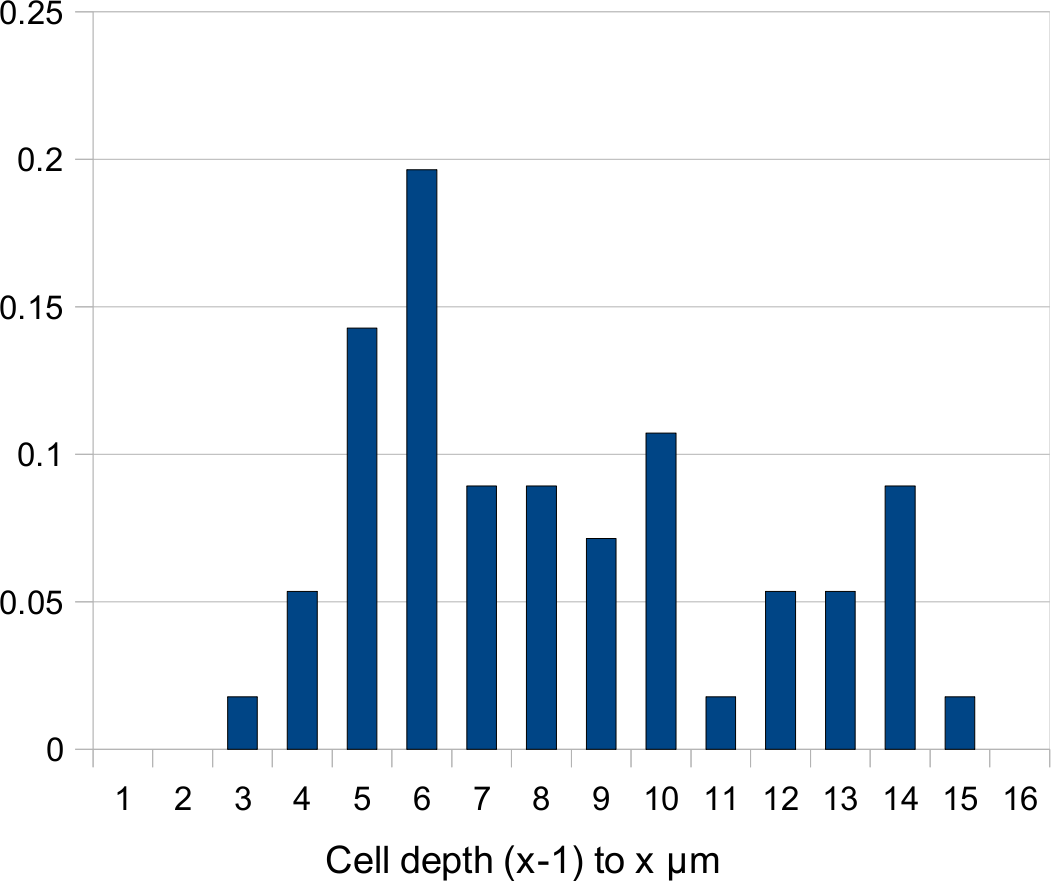
\includegraphics[width=3in]{consistency-cell-depth-distribution.png}
	\end{center}
	%\label{fig:cell-depth-distribution}
\end{figure}

In flat mounts, i.e.\ in the AP/DV plane, it is possible to measure the \textbf{mitotic index} as the number of PH3+ cells per unit area $m_d$. If PH3 only stains for a period of time $\tau_\textrm{mitosis}$, we may calculate the division rate as $$\lambda_d = \frac{\rho_d}{\tau_\textrm{mitosis}}\frac{m_d s [DV]_d}{p_d},$$ where $\rho_d$ is the proportion of progenitor cells in domain $d$, e.g.\ from the preliminary data, $\rho_d \simeq 1$. In practice, we do not know $\tau_\textrm{mitosis}$, though it is should be a constant of time and space; however, it is conceivable that $\rho_d$ may change through changes in $\lambda$, $\gamma$, $r_1$ or $r_2$ (in fact, may be quite generally a functional on their values for all previous times). From the data so far, we can see the change in $\lambda_d \tau_\textrm{mitosis} / \rho_d$:

\begin{figure}[h]
	\begin{center}
		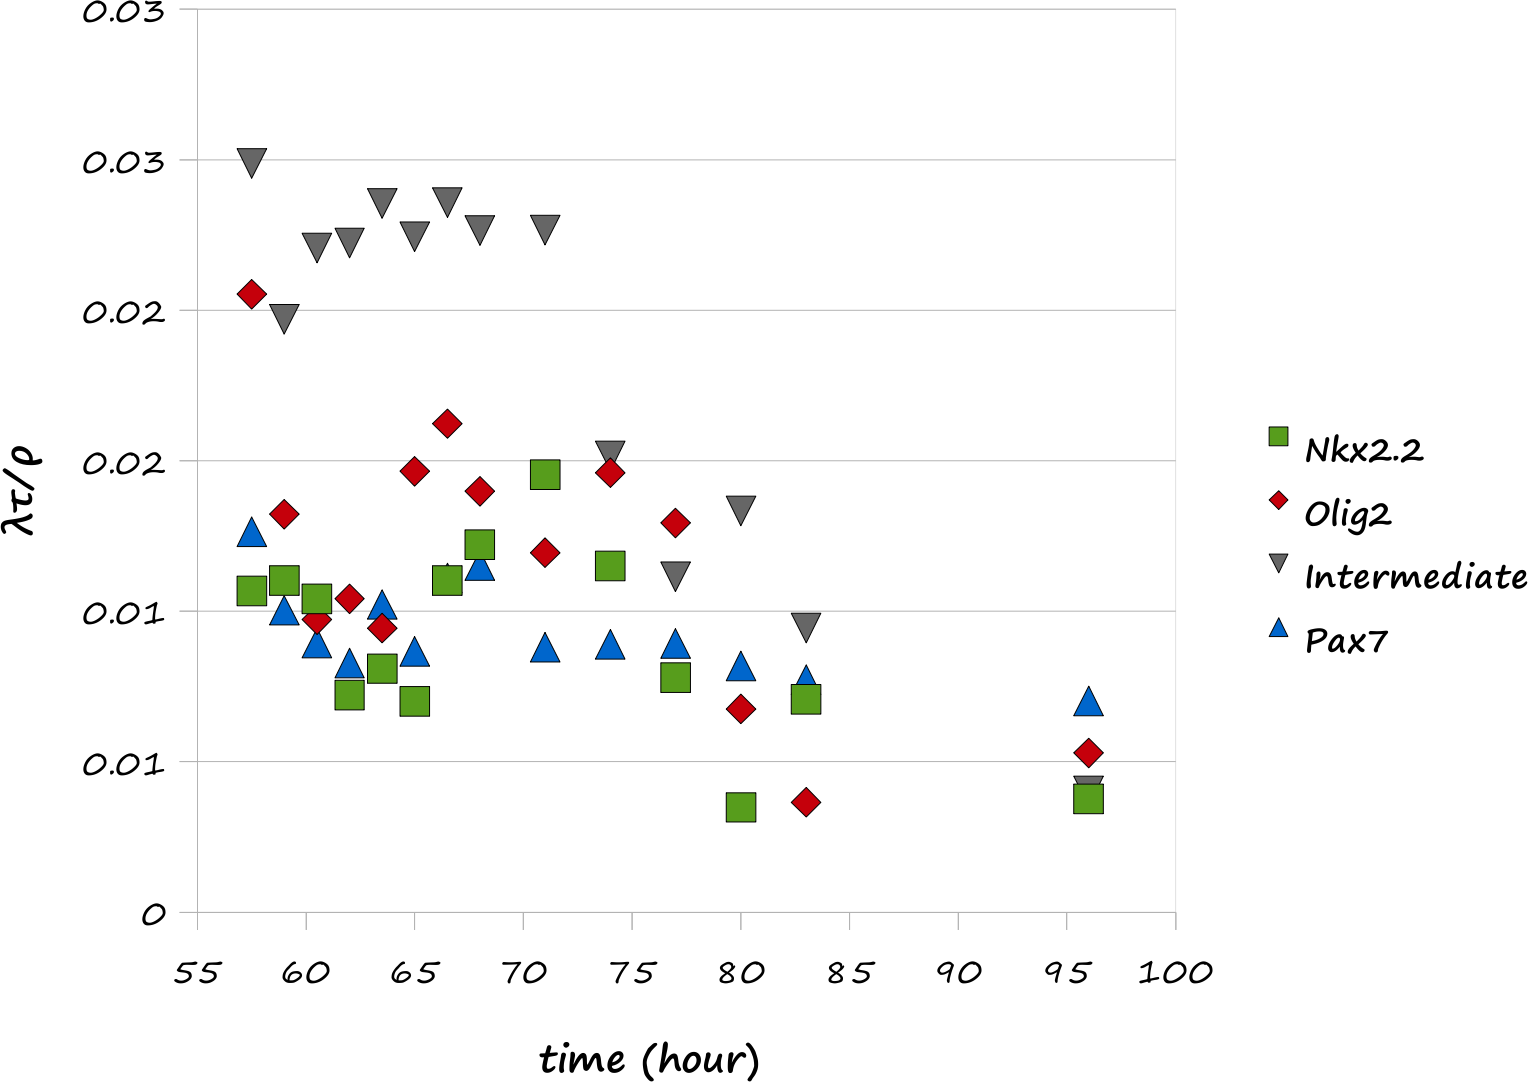
\includegraphics[width=4in]{consistency-mitotic-index.png}
	\end{center}
	%\label{fig:mitotic-index}
\end{figure}


Assuming a PH3 staining time $\tau_\textrm{mitosis} = \SI{15}{\minute}$ and $\rho_d = 1$ we find that a cell division time $1/\lambda_d \simeq \SI{25}{\hour}$, at least before $t \le \SI{75}{\hour}$. There is, however, a definite drop afterwards. Could this be due to a changing $\rho_d$?

To come: corrected progenitor counts; theoretical growth rates and clonal fate analysis.

\end{document}
